\documentclass[tikz,border=10pt]{standalone}
\usepackage{tikz}
\usetikzlibrary{shapes,arrows,positioning,calc,patterns,shadows,arrows.meta}

\definecolor{bertblue}{RGB}{66,133,244}
\definecolor{gptgreen}{RGB}{52,168,83}
\definecolor{soscolor}{RGB}{251,188,5}
\definecolor{tokencolor}{RGB}{142,36,245}

\begin{document}
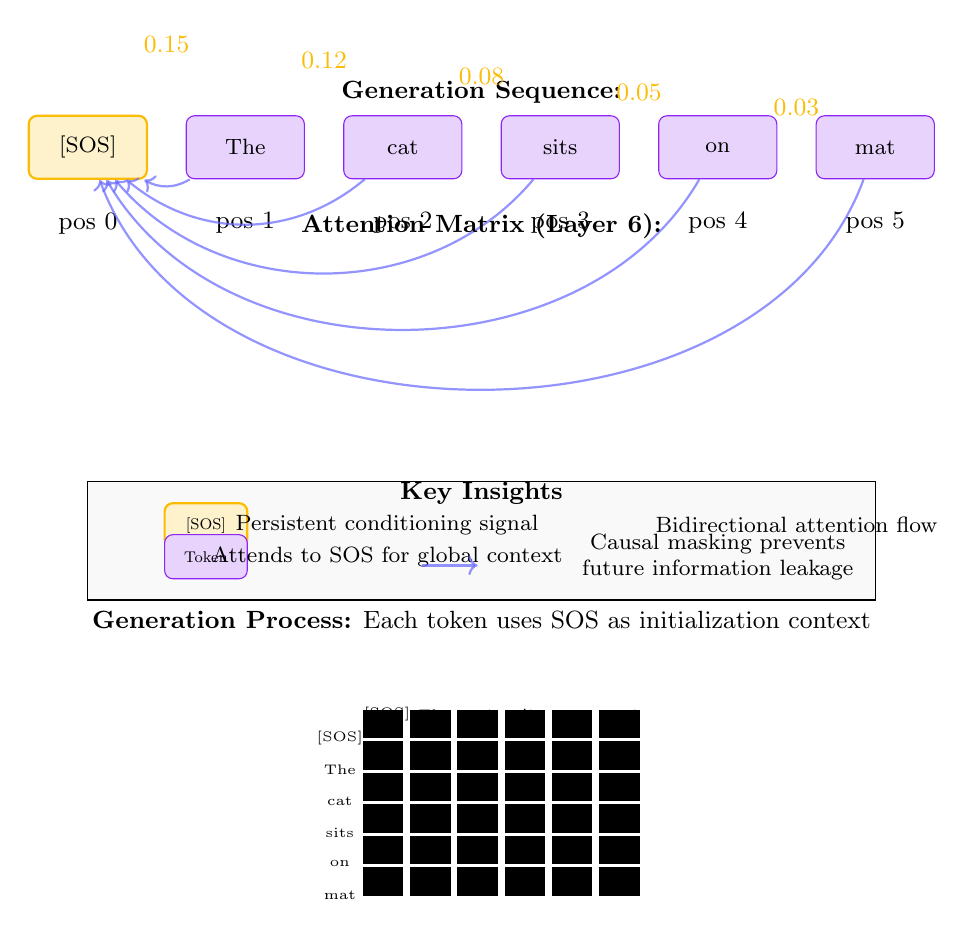
\begin{tikzpicture}[
    token/.style={rectangle, rounded corners=3pt, minimum width=1.5cm, minimum height=0.8cm, font=\footnotesize},
    sostoken/.style={token, fill=soscolor!20, draw=soscolor, thick},
    normaltoken/.style={token, fill=tokencolor!20, draw=tokencolor},
    attention/.style={->, thick, blue!60, opacity=0.7},
    label/.style={font=\small},
    title/.style={font=\large\bfseries}
]

% Title removed - using figure caption instead

% Input sequence with SOS
\node[label] at (6, 7.2) {\textbf{Generation Sequence:}};

% Tokens
\node[sostoken] (sos) at (1, 6.5) {[SOS]};
\node[normaltoken] (t1) at (3, 6.5) {The};
\node[normaltoken] (t2) at (5, 6.5) {cat};
\node[normaltoken] (t3) at (7, 6.5) {sits};
\node[normaltoken] (t4) at (9, 6.5) {on};
\node[normaltoken] (t5) at (11, 6.5) {mat};

% Position labels
\node[label, below=0.3cm of sos] {pos 0};
\node[label, below=0.3cm of t1] {pos 1};
\node[label, below=0.3cm of t2] {pos 2};
\node[label, below=0.3cm of t3] {pos 3};
\node[label, below=0.3cm of t4] {pos 4};
\node[label, below=0.3cm of t5] {pos 5};

% Attention arrows from subsequent tokens to SOS
\draw[attention] (t1) to[bend left=30] (sos);
\draw[attention] (t2) to[bend left=40] (sos);
\draw[attention] (t3) to[bend left=50] (sos);
\draw[attention] (t4) to[bend left=60] (sos);
\draw[attention] (t5) to[bend left=70] (sos);

% Attention weights (example values)
\node[label, soscolor] at (2, 7.8) {0.15};
\node[label, soscolor] at (4, 7.6) {0.12};
\node[label, soscolor] at (6, 7.4) {0.08};
\node[label, soscolor] at (8, 7.2) {0.05};
\node[label, soscolor] at (10, 7.0) {0.03};

% Self-attention pattern visualization
\node[label] at (6, 5.5) {\textbf{Attention Matrix (Layer 6):}};

% Create attention matrix
\begin{scope}[shift={(6,-1)}]
\foreach \i in {0,...,5} {
    \foreach \j in {0,...,5} {
        \pgfmathsetmacro{\opacity}{0.8 - 0.1*\j}
        \ifnum\j=0
            \def\color{soscolor}
        \else
            \def\color{tokencolor}
        \fi
        \ifnum\i=0
            \fill[\color!\opacity!white] (\j*0.6-1.5, -\i*0.4) rectangle ++(0.5, 0.35);
        \else
            \ifnum\j<\i
                \pgfmathsetmacro{\attweight}{0.8 - 0.1*(\i-\j)}
                \fill[blue!\attweight!white] (\j*0.6-1.5, -\i*0.4) rectangle ++(0.5, 0.35);
            \else
                \fill[gray!10] (\j*0.6-1.5, -\i*0.4) rectangle ++(0.5, 0.35);
            \fi
        \fi
        \draw[thin] (\j*0.6-1.5, -\i*0.4) rectangle ++(0.5, 0.35);
    }
}

% Matrix labels
\node[label, font=\tiny] at (-1.8, 0) {[SOS]};
\node[label, font=\tiny] at (-1.8, -0.4) {The};
\node[label, font=\tiny] at (-1.8, -0.8) {cat};
\node[label, font=\tiny] at (-1.8, -1.2) {sits};
\node[label, font=\tiny] at (-1.8, -1.6) {on};
\node[label, font=\tiny] at (-1.8, -2.0) {mat};

\node[label, font=\tiny] at (-1.2, 0.3) {[SOS]};
\node[label, font=\tiny] at (-0.6, 0.3) {The};
\node[label, font=\tiny] at (0, 0.3) {cat};
\node[label, font=\tiny] at (0.6, 0.3) {sits};
\node[label, font=\tiny] at (1.2, 0.3) {on};
\node[label, font=\tiny] at (1.8, 0.3) {mat};
\end{scope}

% Legend
\node[rectangle, draw=black, fill=gray!5, minimum width=10cm, minimum height=1.5cm] at (6, 1.5) {};
\node[label, font=\small\bfseries] at (6, 2.1) {Key Insights};

\node[sostoken, scale=0.7] at (2.5, 1.7) {[SOS]};
\node[label, font=\footnotesize] at (4.8, 1.7) {Persistent conditioning signal};

\node[normaltoken, scale=0.7] at (2.5, 1.3) {Token};
\node[label, font=\footnotesize] at (4.8, 1.3) {Attends to SOS for global context};

\draw[attention, scale=0.7] (7.5, 1.7) -- (8.5, 1.7);
\node[label, font=\footnotesize] at (10, 1.7) {Bidirectional attention flow};

\node[label, font=\footnotesize, align=center] at (9, 1.3) {Causal masking prevents\\future information leakage};

% Generation flow
\node[label] at (6, 0.5) {\textbf{Generation Process:} Each token uses SOS as initialization context};

\end{tikzpicture}
\end{document}